\documentclass[t,aspectratio=169,usenames,dvipsnames,xcolor=table]{beamer}
\usepackage{redhat-beamer/redhat}
\usepackage{layout}
\usepackage{xcolor}
\usepackage{ulem}
\usepackage{pifont}
\usepackage{makecell}


\definecolor{hlcolor}{RGB}{2,65,77}
\definecolor{bgcolor}{RGB}{241,241,241}
\definecolor{rhreddark}{RGB}{163,0,0}

\newcommand{\hll}[1]{{\color{rhrednew} #1}}
\newcommand{\hl}[1]{\textbf{\hll{#1}}}

%
% font
%
\usepackage{fontspec}
\usepackage{fontawesome}
\setmonofont{FreeMono}

\usepackage{tikz}
\usetikzlibrary{positioning,calc}

\usepackage{listings}
\usepackage{lstautogobble}
\lstset{
    language=C,
    basicstyle={\tiny\ttfamily},
    autogobble=true,
    moredelim=**[is][\only<1>{\color{rhrednew}\bfseries}]{^}{^},
    moredelim=**[is][\only<2->{\color{rhrednew}\bfseries}]{@}{@},
    moredelim=**[is][\only<2->{\color{blue}\bfseries}]{~}{~},
}

\renewcommand<>{\sout}[1]{
  \alt#2{\beameroriginal{\sout}{#1}}{#1}
}

\tikzset{onslide/.code args={<#1>#2}{%
  \only<#1>{\pgfkeysalso{#2}} % \pgfkeysalso doesn't change the path
}}

\title{Advanced Git}
\subtitle{IVS demonstration exercise}
\author{Viktor Malík \and Petr Stodůlka \and Pavel Odvody}
\institute{Red Hat}
\date{April 14, 2020}

\begin{document}

\maketitle

\begin{frame}
  \frametitle{Prerequisites}
  \begin{itemize}
    \setlength\itemsep{.3em}
    \item Basic knowledge of Git commands for:
      \begin{itemize}
      \setlength\itemsep{.3em}
        \item creating commits (\texttt{git add, git commit})
        \item inspecting current state (\texttt{git status, git diff})
        \item inspecting history (\texttt{git log, git show})
        \item working with remotes (\texttt{git pull, git push})
        \item working with branches (\texttt{git checkout, git branch})
      \end{itemize}
  \end{itemize}
\end{frame}

\section{``Advanced'' work with Git}

\begin{frame}
  \frametitle{Let's start}
  \begin{itemize}
    \setlength\itemsep{.5em}
    \item We'll write a simple tool for counting characters, words, and lines
      in a file (similar to the \texttt{wc} utility)
    \item We start with a pre-initialized repo containing very basics of the
      tool:\\
      \url{https://github.com/viktormalik/git-workshop}
    \item The repo contains a source file \texttt{wc.c}, a testing file, and 
      a \texttt{Makefile}
    \item We start by adding \texttt{.gitignore} and commiting it
  \end{itemize}
\end{frame}

\begin{frame}
  \frametitle{Current status of the repo}
  \centering
  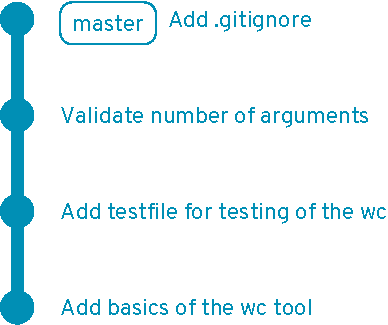
\includegraphics[scale=0.8]{../git-figures/01-initial.pdf}
\end{frame}

\begin{frame}
  \frametitle{Basic team synchronisation}
  \vspace{-1em}
  Every member implements a different feature in their \textit{master}
  \vspace{1em}
  \begin{center}
    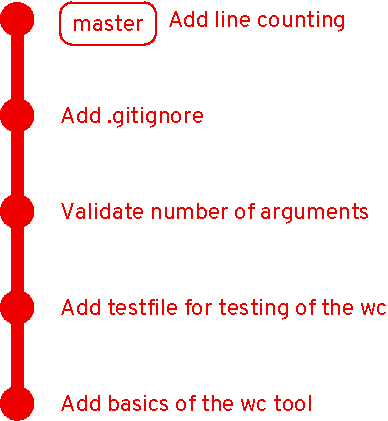
\includegraphics[scale=0.6]{../git-figures/02-lines.pdf}
    \hspace{6em}
    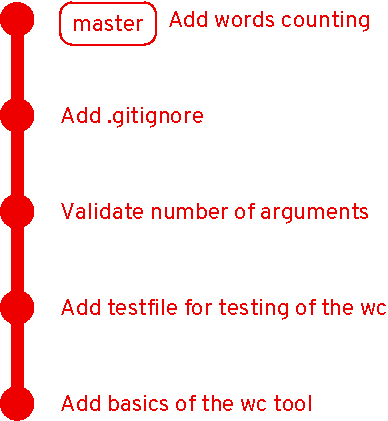
\includegraphics[scale=0.6]{../git-figures/02-words.pdf}
  \end{center}
\end{frame}

\begin{frame}
  \frametitle{Basic team synchronisation}
  \vspace{-1em}
  The second one to push must do a merge (and resolve a merge conflict)
  \vspace{1em}
  \begin{center}
    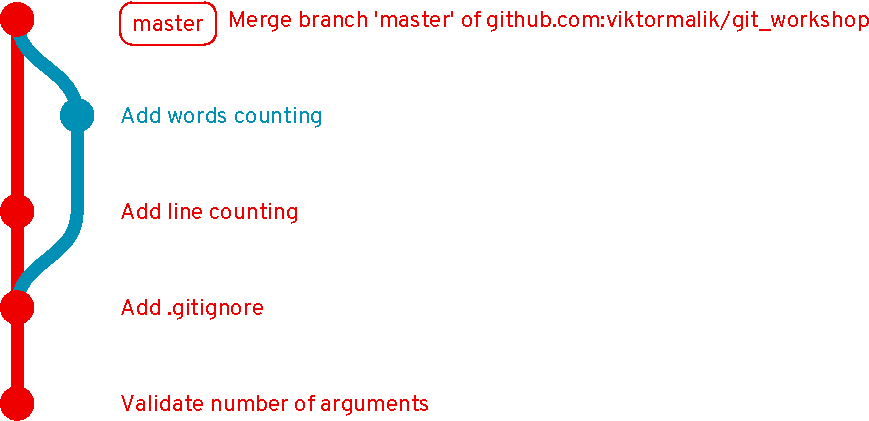
\includegraphics[scale=0.6]{../git-figures/02-after-merge.pdf}
  \end{center}
\end{frame}

\begin{frame}
  \frametitle{Better team synchronisation}
  \begin{itemize}
    \setlength\itemsep{.5em}
    \item \textbf{This is not a good practice!}
    \item Always implement new features in \textbf{separate branches}.
    \item Potential merge conflicts should be resolved in the feature branch.
    \item Ideally, merging into master should be always done using \textbf{pull
      requests}
      \begin{itemize}
        \setlength\itemsep{.2em}
        \item They allow other team members to comment on the changes
        \item Changes can be \textbf{reviewed} before they get into master
        \item Master always contains a working and approved version of the
          project
      \end{itemize}
  \end{itemize}
\end{frame}

\begin{frame}
  \frametitle{Using a feature branch}
  \vspace{-1em}
  Let us add help into the tool using a separate branch \textit{add\_help}
  \vspace{1em}
  \begin{center}
    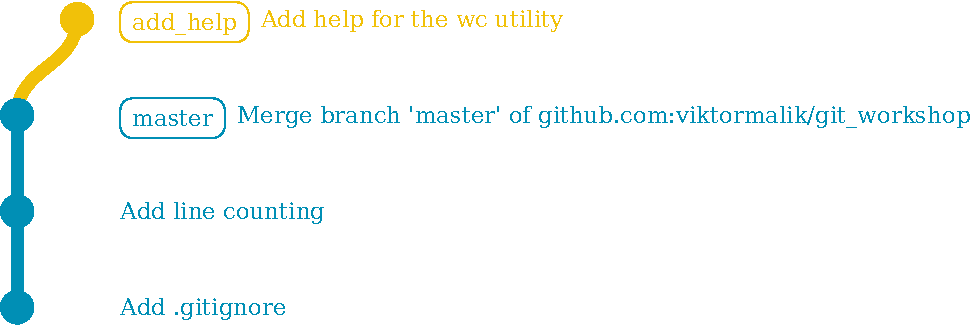
\includegraphics[scale=0.6]{../git-figures/03-help.pdf}
  \end{center}
\end{frame}

\begin{frame}
  \frametitle{Using a feature branch}
  \vspace{-1em}
  The state of \textit{master} after \textbf{rebase}:
  \vspace{1em}
  \begin{center}
    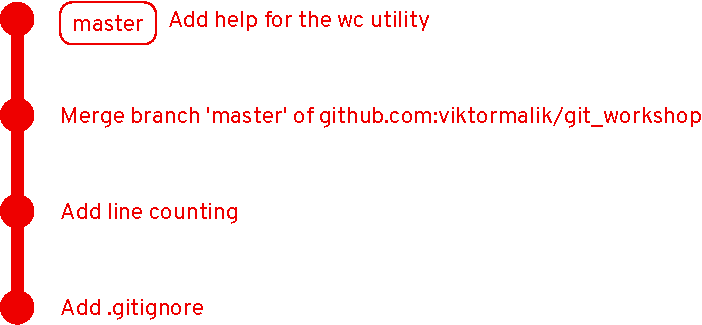
\includegraphics[scale=0.6]{../git-figures/03-after-rebase.pdf}
  \end{center}
\end{frame}

\begin{frame}
  \frametitle{Moving branches}
  \vspace{-1em}
  We have 2 branches pointing to the same commit and we want to move one
  backwards.
  \vspace{1em}
  \begin{center}
    \hspace{-2em}
    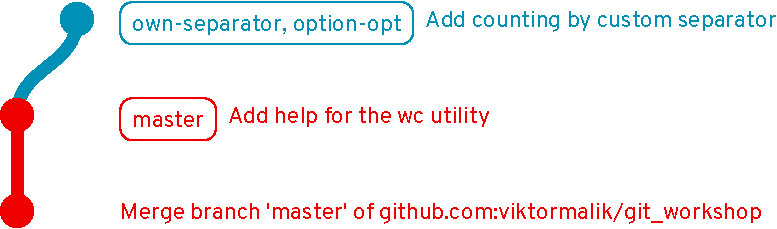
\includegraphics[scale=0.7]{../git-figures/04-start.pdf}
  \end{center}
\end{frame}

\begin{frame}
  \frametitle{Moving branches}
  \vspace{-1em}
  This can be done using\, \texttt{git reset HEAD \^}
  \vspace{1em}
  \begin{center}
    \hspace{-2em}
    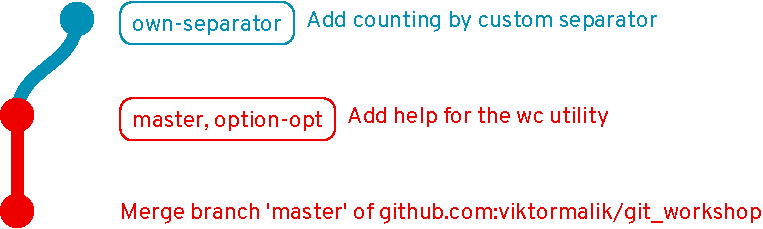
\includegraphics[scale=0.7]{../git-figures/04-after-reset.pdf}
  \end{center}
\end{frame}

\begin{frame}
  \frametitle{Moving branches}
  \vspace{-1em}
  After adding a new commit to \textit{options-opt}:
  \vspace{1em}
  \begin{center}
    \hspace{-2em}
    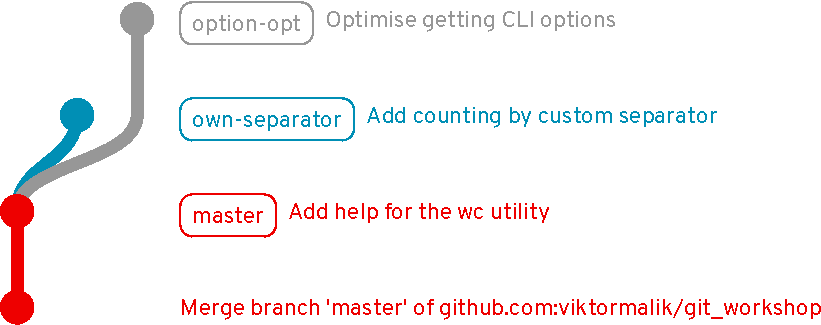
\includegraphics[scale=0.6]{../git-figures/04-separate-branches.pdf}
  \end{center}
\end{frame}

\begin{frame}
  \frametitle{Moving branches}
  \vspace{-1em}
  \textit{options-opt} can be now merged into master while
    \textit{own-separator} remains a feature branch in development.
  \vspace{1em}
  \begin{center}
    \hspace{-2em}
    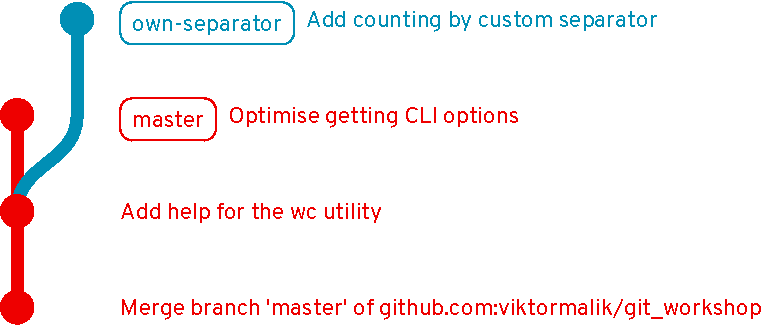
\includegraphics[scale=0.6]{../git-figures/04-after-merge.pdf}
  \end{center}
\end{frame}

\begin{frame}
  \frametitle{Rebasing feature branches}
  \vspace{-1em}
  We add more commits to the feature branch and then \textbf{rebase} it onto
  \textit{master} (to avoid creation of a merge commit).
  \vspace{1em}
  \begin{center}
    \hspace{-2em}
    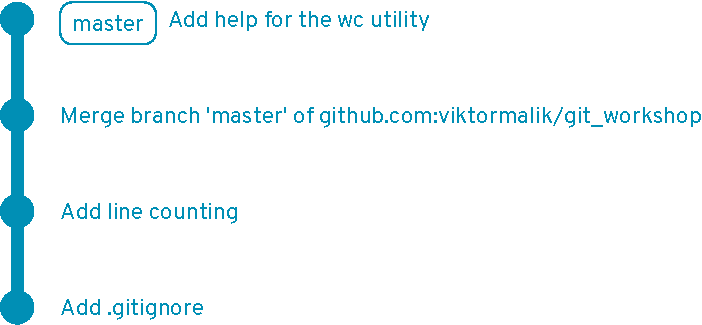
\includegraphics[scale=0.6]{../git-figures/04-after-rebase.pdf}
  \end{center}
\end{frame}

\begin{frame}
  \frametitle{Rebasing feature branches}
  \vspace{-1em}
  We made a mistake during the rebase, which we had to fix with an additional
  commit.
  \vspace{1em}
  \begin{center}
    \hspace{-2em}
    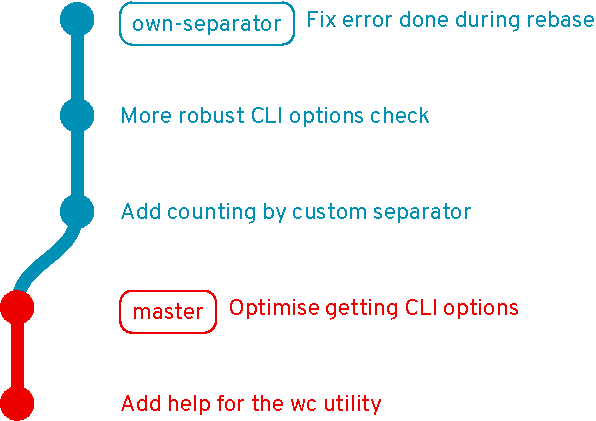
\includegraphics[scale=0.6]{../git-figures/04-after-fix.pdf}
  \end{center}
\end{frame}

\begin{frame}
  \frametitle{Rebasing feature branches}
  \vspace{-1em}
  It is possible to merge the ``fix commit'' into one of the previous commits
  using \textbf{interactive rebase} (\texttt{git rebase -i}).
  \vspace{1em}
  \begin{center}
    \hspace{-2em}
    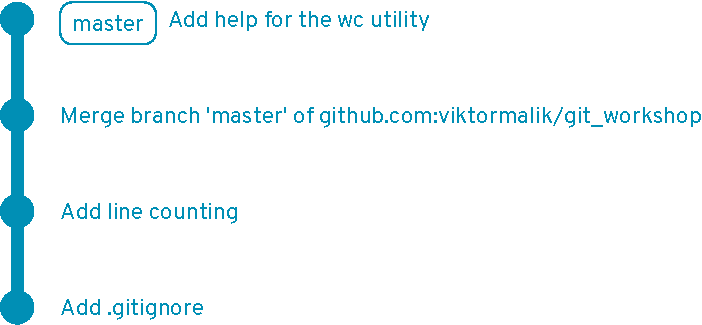
\includegraphics[scale=0.6]{../git-figures/04-after-rebase.pdf}
  \end{center}
\end{frame}

\begin{frame}
  \frametitle{Interactive rebase}
  \begin{itemize}
    \setlength\itemsep{.5em}
    \item One of the most important Git features in the modern pull
      request-based workflow.
    \item Allows to \textbf{edit}, \textbf{reorder}, \textbf{merge (squash)},
      or \textbf{drop} commits.
    \item \textbf{Rewrites history} -- should be only used on feature branches.
    \item \textbf{Never rewrite history of master!}
      \begin{itemize}
        \item Other developers would not be able to do\, \texttt{git pull}.
      \end{itemize}
  \end{itemize}
\end{frame}

\begin{frame}
  \frametitle{Copying commits from other branches}
  \vspace{-1em}
  It is possible to copy commits from other branches (e.g. commits implementing
  useful features from co-workers feature branches) using\, \texttt{git
  cherry-pick}.
  \vspace{1em}
  \begin{center}
    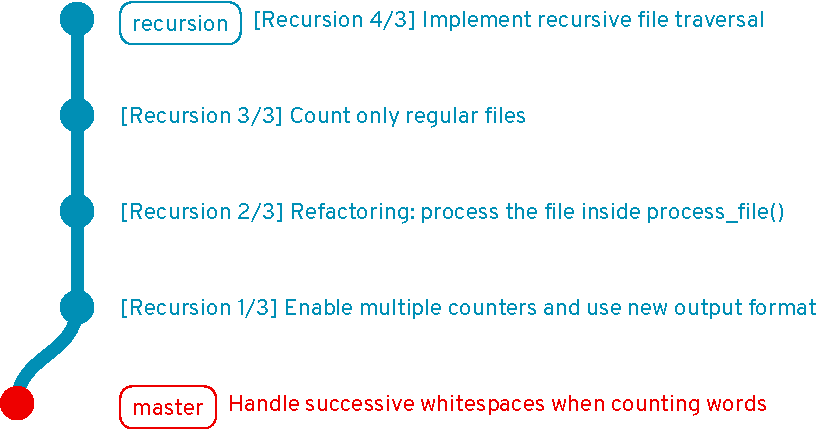
\includegraphics[scale=0.6]{../git-figures/05-recursion.pdf}
  \end{center}
\end{frame}

\begin{frame}
  \frametitle{Copying commits from other branches}
  \vspace{-1em}
  After moving 3 commits from \textit{recursion} into \textit{multiple-files}:
  \vspace{2.2em}
  \begin{center}
    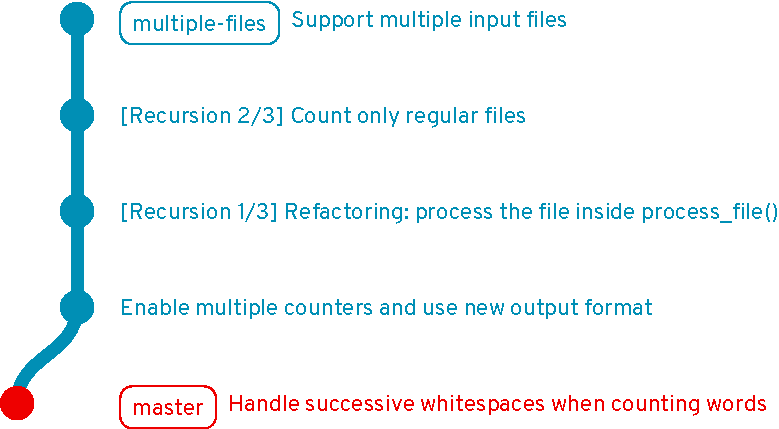
\includegraphics[scale=0.6]{../git-figures/05-multiple-files.pdf}
  \end{center}
\end{frame}

\begin{frame}
  \frametitle{Copying commits from other branches}
  \vspace{-1em}
  If the commits are altered in \textit{multiple-files}, it may be needed to
  use \texttt{skip} when rebasing \textit{recursion} onto
  \textit{multiple-files}.
  \vspace{1em}
  \begin{center}
    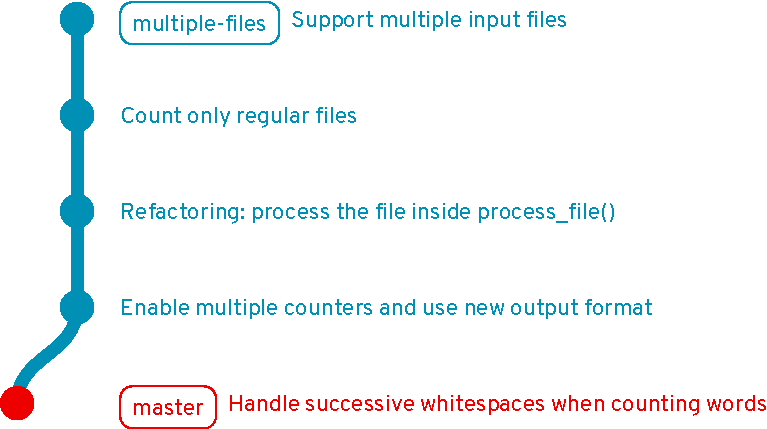
\includegraphics[scale=0.6]{../git-figures/05-multiple-files-rebase.pdf}
  \end{center}
\end{frame}

\begin{frame}
  \frametitle{Hunting bugs in Git history}
  \vspace{-1em}
  \begin{itemize}
    \setlength\itemsep{.5em}
    \item We often discover a bug that was certainly introduced
      \textbf{somewhere in the Git history}.
      \begin{itemize}
        \item There is a revision in the past where certain test works correctly.
        \item However, the test does not work now.
      \end{itemize}
    \pause
    \item Git offers \texttt{git bisect} that uses \textbf{binary search} to
      localise the commit that caused the bug.
      \begin{itemize}
        \item \texttt{git bisect start }starts bisecting.
        \item \texttt{git bisect good }marks a commit that does not contain
          the bug.
        \item \texttt{git bisect bad }marks a commit contains the bug.
        \item \texttt{git bisect skip }marks a commit that cannot be evaluated.
      \end{itemize}
    \pause
    \item The process can be \textbf{automated} using a script that returns 0
      on success and a non-zero result on failure.
  \end{itemize}
\end{frame}

\section{Git tips and tricks}

\begin{frame}
  \frametitle{Cloning repositories with a long history}
  \begin{itemize}
    \setlength\itemsep{.5em}
    \item If a repo has a long history, it may take long time to clone it.
    \item If the entire history is no needed, it is possible to use a
      \textbf{shallow copy}:\\ \texttt{git clone --max-depth N}
    \item Try it with the Linux kernel:\\
      \texttt{git clone --max-depth 1 https://github.com/torvalds/linux}
  \end{itemize}
\end{frame}

\begin{frame}
  \frametitle{Default push and pull into different remotes}
  \begin{itemize}
    \setlength\itemsep{.5em}
    \item When using pull requests, it may be useful to pull from the
      \textbf{upstream} repo but push into own \textbf{fork}.
    \item A different remote for push can be configured using:\\
      \texttt{git config remote.pushdefault <remote>}
    \item Alternatively, this can be configured per-branch:\\
      \texttt{git config branch.<branch>.pushremote <remote>}
  \end{itemize}
\end{frame}

\begin{frame}
  \frametitle{Signing commits}
  \begin{itemize}
    \setlength\itemsep{.5em}
    \item By default, it is not possible to verify that a certain commit was
      truly created by the person who is stated as the author.
    \item Theoretically, anyone can set your name and email as theirs and
      commit on your behalf.
    \pause
    \item To resolve this problem, Git offers \textbf{signing commits} using
      GPG keys.
    \item GitHub offers a nice tutorial on how to setup commit signing:
      \url{https://help.github.com/en/github/authenticating-to-github/signing-commits}
  \end{itemize}
\end{frame}

\begin{frame}
  \frametitle{Setup your environment}
  \vspace{-2em}
  There are various possibilities on how to ease your life with Git:
  \begin{itemize}
    \setlength\itemsep{.5em}
    \item \textbf{Git prompt}
      \begin{itemize}
        \item It is possible to setup Bash prompt such that it shows the
          current branch, state of the directory, etc.
        \item There are many tutorials on how to set the prompt
        \item Some alternative shells (e.g. Fish, zsh) include Git prompt by
          default
      \end{itemize}
    \pause
    \item \textbf{IDE/Editor support}
      \begin{itemize}
        \item It is useful to see which lines were added/removed/changed from
          HEAD.
        \item Most IDEs and editors offer a way to setup this.
      \end{itemize}
    \pause
    \item \textbf{Use tools for history inspection}
      \begin{itemize}
        \item There is a number of tools for an easier history traversal
        \item E.g. \textbf{tig}, gitk, \ldots
      \end{itemize}
  \end{itemize}
\end{frame}

\begin{frame}[fragile]
  \frametitle{Setup your environment}
  \vspace{-1em}
  \begin{itemize}
    \setlength\itemsep{.5em}
    \item \textbf{Command aliases}
      \begin{itemize}
        \setlength\itemsep{.5em}
        \item Many Git commands are quite long (or have many options).
        \item It is possible to setup short aliases for most commonly used
          commands.
        \item Git offers a way to set aliases:\\
          \texttt{git config --global alias.co checkout\\...}\\
          or edit \texttt{\$HOME/.gitconfig}:\\
          \texttt{
            [alias]\\
            \quad co = checkout\\
            \quad ...}
        \item An alternative is to setup aliases via shell
      \end{itemize}
  \end{itemize}
\end{frame}

\begin{frame}
  \frametitle{Useful links}
  \begin{itemize}
    \item Atlassian Advanced Git Tutorials\\
      \url{https://www.atlassian.com/git/tutorials/advanced-overview}
    \item GitHub Guides\\
      \url{https://guides.github.com}
    \item GitHub Help\\
      \url{https://help.github.com/en/github}
  \end{itemize}
\end{frame}

\begin{frame}
  \frametitle{TL;DR}
  What you should take out of this talk:
  \begin{itemize}
    \item Learn and practice \textbf{interactive rebase}
    \item \textbf{Read what Git tells you}, there are often good hints (e.g.
      for undoing things)
    \item Keep \textit{master} in good shape
  \end{itemize}
  \setbeamerfont{thankyou}{size=\fontsize{19pt}{2pt}}
  \vspace*{3em}
  \centering
  \usebeamerfont{thankyou}\hl{Thank you for the attention!\\[.5em]Questions?}
\end{frame}

\end{document}
